\section{One-Shot Extends to Multi-Teacher OPD}
% 16 Diverse Queries Remain Sufficient in Multi-Teacher OPD
\label{sec:mopd}

Section~\ref{sec:state-diversity} showed that a small, semantically diverse query set can match full-data OPD within one domain. Modern post-training pipelines often use \emph{multi-teacher on-policy distillation} (MOPD)~\citep{xiao2026mimo,xu2026deepseek}, where one student is trained on several domains in a single run and each query is routed to its domain teacher. This section asks \textit{whether the same query-diversity result carries over: can a small, diverse query set for each domain match full-data MOPD?}

\begin{tcolorbox}[takeawaysbox]
% \begin{itemize}[topsep=0pt, partopsep=0pt, leftmargin=12pt, itemsep=0pt]
%     \item 
    16 semantically diverse queries within each domain are sufficient to match full-data MOPD, which reaches nearly the same average validation accuracy as separate full-data OPD.
% \end{itemize}
\end{tcolorbox}

\begin{figure}[t]
    \centering
    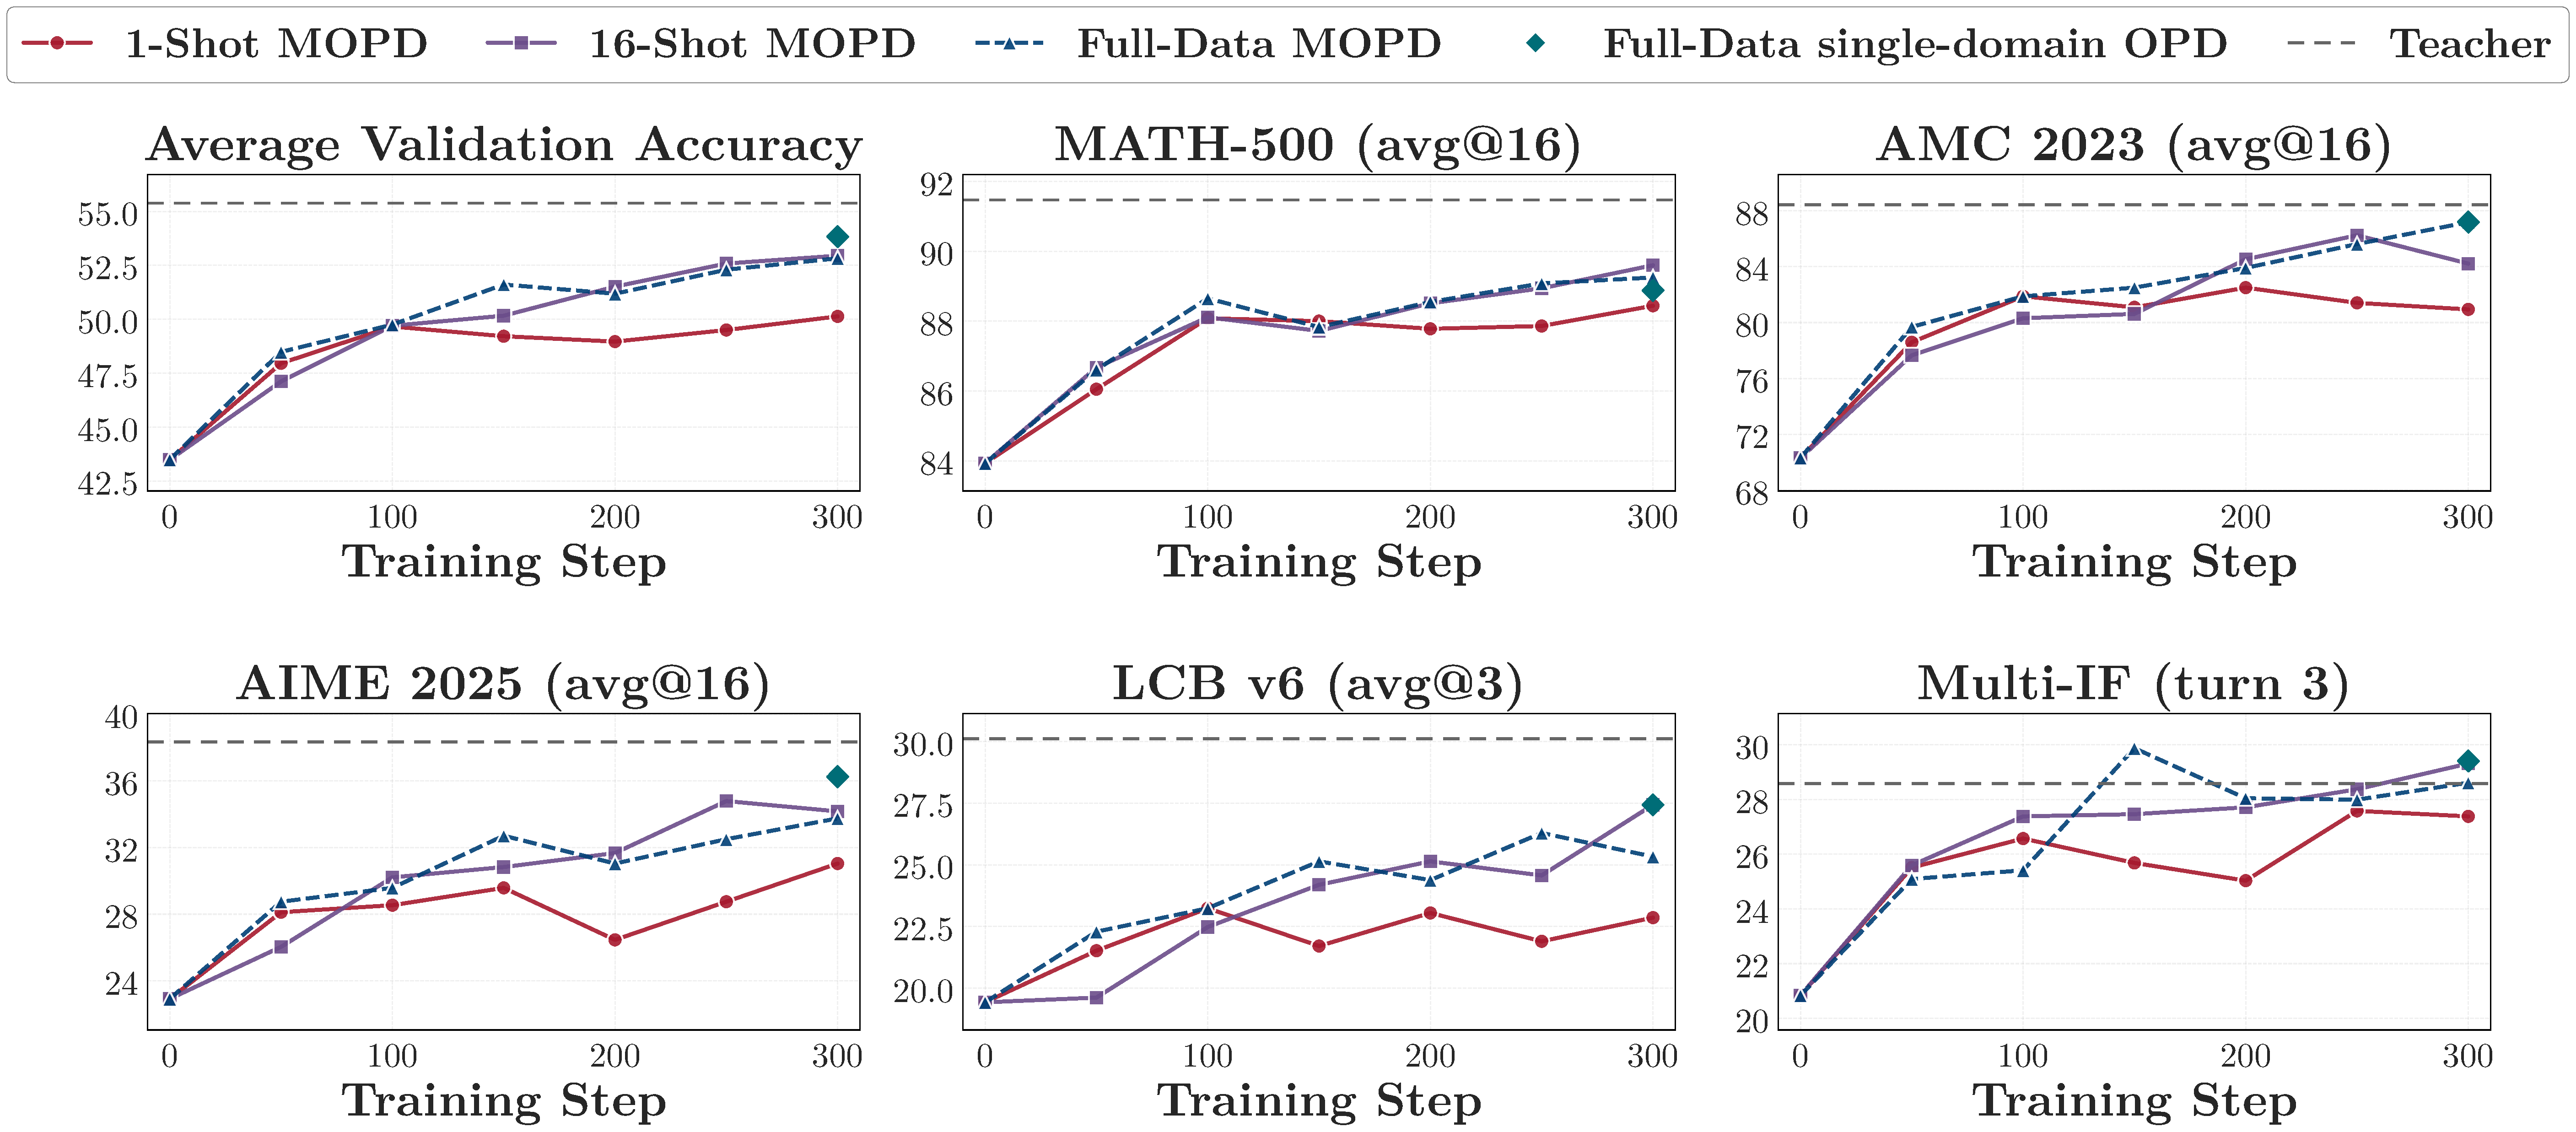
\includegraphics[width=\textwidth]{figures/6_mopd_curves.pdf}
    \caption{
    Validation accuracy of one-shot, 16-shot, and full-data MOPD.
    }
    \label{fig:mopd}
\end{figure}

\paragraph{Setup.}
We train one R1-Distill-1.5B student with MOPD on mathematical reasoning, code generation, and instruction following. The domain teachers from Section~\ref{sec:setup} are JustRL-1.5B for mathematics, Nemotron-1.5B for code, and UltraData-IF-1.5B for instruction following. We exclude agentic tool use because it uses a different student, Qwen-Coder-1.5B. The three settings are one-shot, 16-shot, and full-data MOPD. As in Section~\ref{sec:state-diversity}, the 16-shot setting selects one representative from each of 16 BGE-M3~\citep{chen2024bge} semantic clusters fitted separately within each domain. All settings run for \(300\) steps with the hyperparameters in Table~\ref{tab:mopd-hyperparams}.

\paragraph{Full-data MOPD matches separate full-data OPD.}
At step \(300\), full-data MOPD raises the average validation accuracy from \(43.5\) to \(52.8\), recovering \(79\%\) of the teacher--student gap. The three corresponding full-data OPD runs reach \(53.8\). This \(1.0\)-point difference shows that MOPD remains effective when all three domains are trained in a single run and establishes full-data MOPD as the reference for the query-diversity comparison below.

\paragraph{16 diverse queries per domain match full-data MOPD.}
Increasing the query count from 1 to 16 per domain raises the average validation accuracy from \(50.1\) to \(52.9\) at step \(300\). Full-data MOPD reaches \(52.8\), so 16-shot MOPD recovers \(101\%\) of full-data MOPD's gain. The result is not driven by one domain: calculated separately, the corresponding proportions are \(93\%\) for mathematics, \(136\%\) for code generation, and \(109\%\) for instruction following. Because 16-shot and full-data MOPD use the same rollout and optimization budgets, expanding each domain's query set beyond 16 diverse queries produces no additional average gain in this setting.

Together, these results are consistent with a state-space account for MOPD: semantically diverse queries can induce complementary states within each domain, allowing 16 queries per domain to match full-data MOPD.


